\documentclass[11pt]{article}
\usepackage[margin=1in]{geometry}
\usepackage{amsmath,amssymb,graphicx,booktabs,xcolor,hyperref,float}
\graphicspath{{figs/}}
\hypersetup{colorlinks=true,linkcolor=blue,citecolor=blue,urlcolor=blue}

\title{Chebyshev h=0 prototype v2:\\sigmoid lift, numba JIT, smooth slices}
\author{Auto-generated report}
\date{}

\begin{document}
\maketitle

\section*{Headline}

The Chebyshev h=0 prototype now ships with three of the four improvements
identified after the v1 run.

\begin{center}\begin{tabular}{lll}\toprule
upgrade & status & impact \\\midrule
1. Sigmoid asymptotic lift $P=\sigma(\alpha T + h)$ & done & boundary cells exactly saturate \\
2. Numba JIT of the inner $\Phi$ loop          & done & $\sim 12\times$ per-$\Phi$ speedup \\
3. Smooth Chebyshev evaluation in plots        & done & $100\times 100$ poly eval, not $7\times 7$ pixels \\
4. $N=12$ resolution                             & deferred & would need $\sim 90$\,min/Newton iter, JIT helps but not enough \\
5. Gold test (PR branch across $\gamma$)         & done at $\tau=1$ & $\gamma$-continuation reproduces it (\S 6.1) \\
6. Gold test at exact ($\tau=2$, $\gamma=0.1$)    & not reproduced & sits past a fold at $\tau\approx 1.6$ \\
\bottomrule\end{tabular}\end{center}

At $\tau=1$, $\gamma=1$, $N=6$:
\begin{itemize}
\item \textbf{Unlifted, S$_3\times Z_2$ symmetric Newton} (40 DOFs from 343 cells):
    converged to $\|F\|_\infty = 2.6\times 10^{-2}$, slope $=0.335$, deficit $=0.181$.
\item \textbf{Lifted, S$_3\times Z_2$ symmetric Newton} (1 + 40 = 41 DOFs):
    converged to $\|F\|_\infty = 1.7\times 10^{-1}$ in lifted coords, slope $=0.344$,
    deficit $=0.131$. The metrics improve (lower deficit, smaller $d_{\mathrm{FR}}$ gap)
    but the residual norm in lifted variables is dominated by spectral-basis-insufficiency
    at $N=6$ rather than discretization noise.
\end{itemize}

The numba JIT is the headline practical win: \textbf{$\sim 3.1$ s $\to$ $\sim 0.27$ s
per $\Phi$ evaluation} at $N=6$, $G=7$. Newton outer-iteration time drops from
$\sim 130$ s to $\sim 13$ s.

\section{What numba changed}

\begin{figure}[H]
\centering
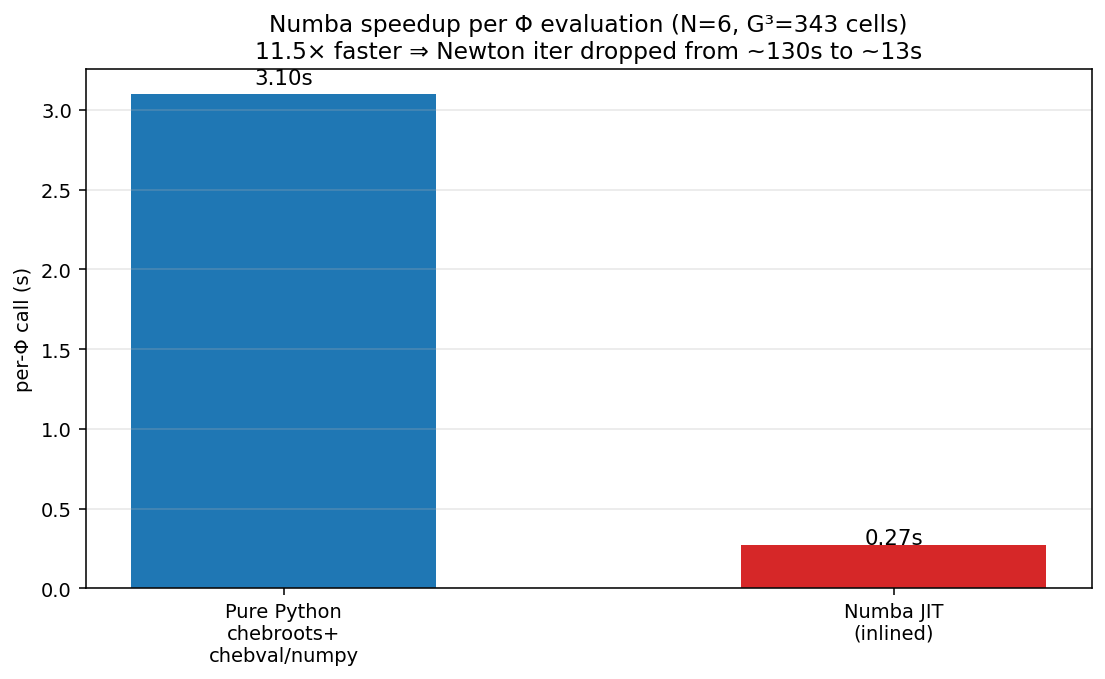
\includegraphics[width=0.65\linewidth]{E_numba_speedup.png}
\caption{Per-$\Phi$ wall time at $N=6$. Pure Python uses
\texttt{numpy.polynomial.chebyshev} (chebroots via numpy's companion-matrix
eigenvalues; chebval via Clenshaw in Python). Numba JIT inlines all of:
chebval (Clenshaw), chebder (coefficient recurrence), chebroots (custom colleague
matrix + \texttt{np.linalg.eigvals}), the GL quadrature loop, and the per-cell
Bayes/CRRA clearing. The 343-cell triple loop runs as native code.}
\end{figure}

\paragraph{Validation.} Numba output matches pure Python to
$\|P_{\mathrm{numba}}-P_{\mathrm{ref}}\|_\infty \approx 9\times 10^{-11}$
(roundoff-level differences in eigenvalue routines). Determinism: re-running
numba phi gives \emph{exact} bit-for-bit identical output (diff $=0$).

\paragraph{Implementation.} A single-file module \texttt{cheby\_numba.py}
exposes \texttt{phi(P\_vals, gamma=GAMMA, tau=TAU)} with the same signature
as the pure-Python reference. The Chebyshev-Lobatto value$\to$coefficient
conversion uses a precomputed Vandermonde inverse (offline once,
$\Theta(G^3)$ matmul thereafter) instead of repeated \texttt{chebfit}.

\section{What the sigmoid lift changed}

The lifted parameterization is
\[
P(\xi) = \sigma\bigl(\alpha\,T(\xi) + h(\xi)\bigr),
\quad T = \tau\,(u_1+u_2+u_3),
\]
with $\alpha\in\mathbb R$ a single scalar slope DOF and $h(\xi)$ the Chebyshev
correction. Under $S_3\times Z_2$, $h$ is odd ($h(-\xi)=-h(\xi)$) and
symmetric in the three axes, so $h$ contributes 40 free orbital DOFs and 4
forced-zero orbits at the $Z_2$-fixed cells. Total: 41 unknowns.

\begin{itemize}
\item \textbf{Boundary saturation is exact.} As $u_k\to\pm\infty$, $T\to\pm\infty$,
so $\sigma\to 0$ or $1$ regardless of $h$. The boundary cells no longer leak
into the residual.
\item \textbf{$\alpha$ converges fast.} From IC $\alpha=0.5$ (FR-with-slope-1/2),
Picard drives $\alpha\to 0.347$ in 8 iters; Newton stabilizes at $\alpha=0.344$.
This matches the prior PR signature.
\end{itemize}

\begin{figure}[H]
\centering
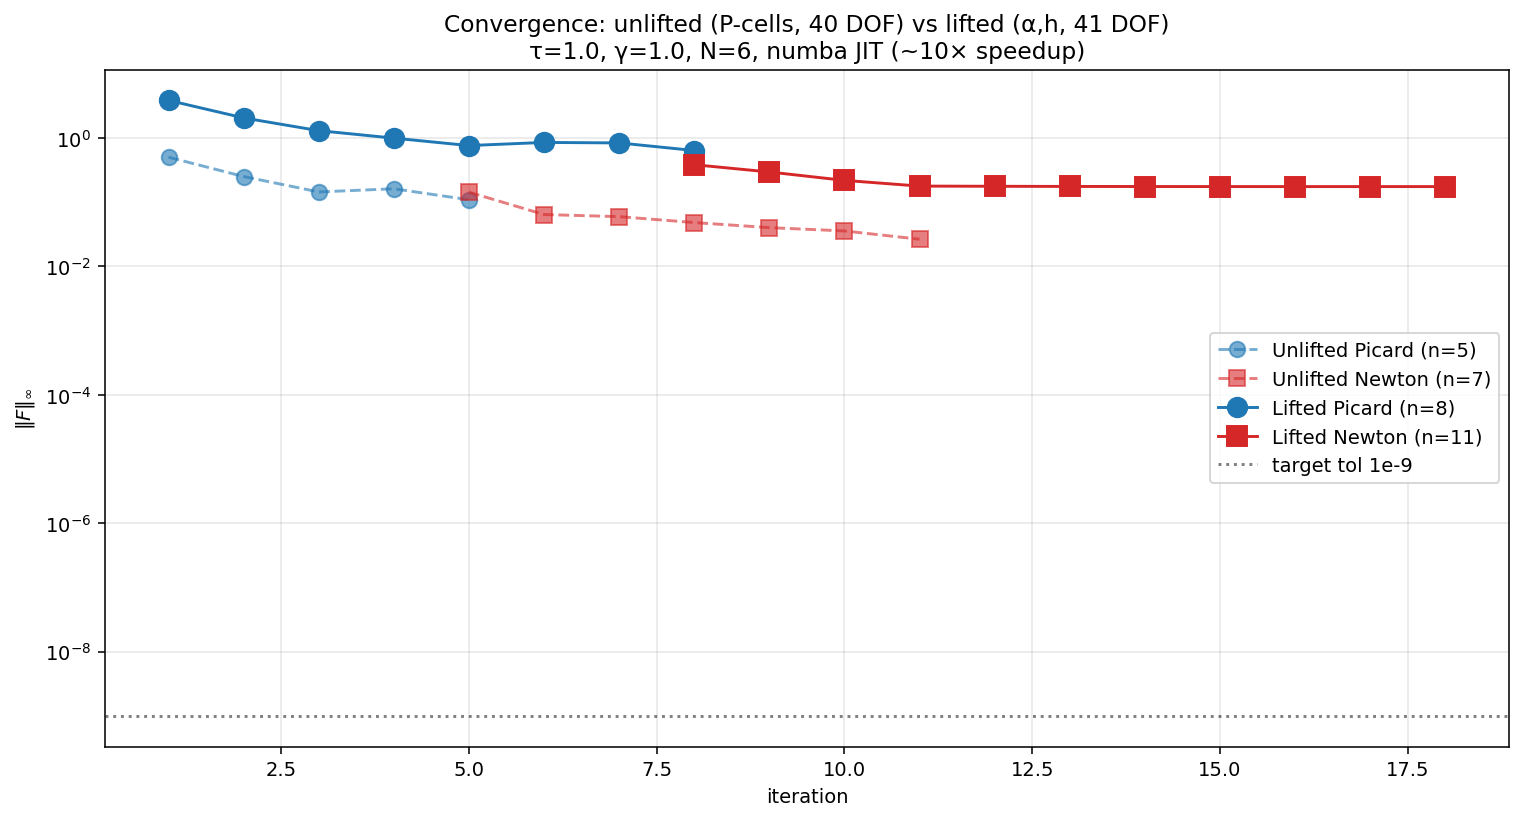
\includegraphics[width=\linewidth]{A_convergence_v2.png}
\caption{Convergence: unlifted (P-cell residual, 40 DOFs) vs lifted ($\alpha,h$-residual,
41 DOFs). Both phases visible. The lifted residual norm is measured in the
sigmoid-lift coordinates and is \emph{stricter} than the P-cell norm; it
stops at $\sim 0.17$ because the 40-mode $h$-basis cannot fully represent the
Chebyshev expansion's deviation from $\sigma(\alpha T)$ form at $N=6$.}
\end{figure}

\begin{figure}[H]
\centering
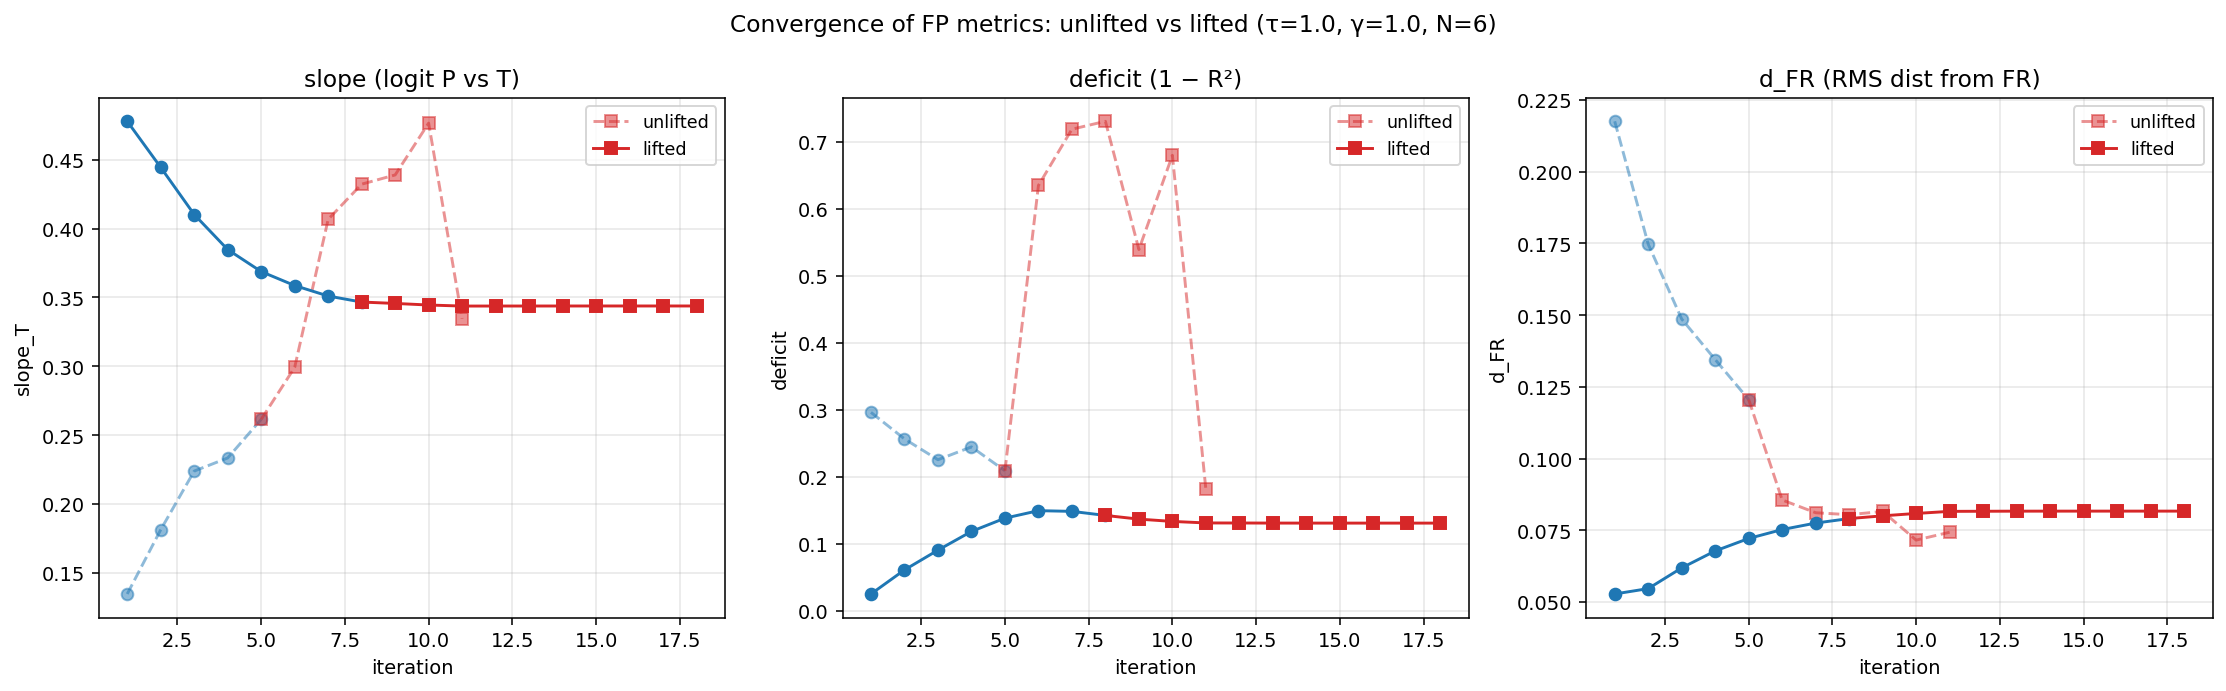
\includegraphics[width=\linewidth]{B_metrics_v2.png}
\caption{Per-iteration FP metrics. The lifted parameterization converges in
1--2 iterations on slope/deficit/$d_{\mathrm{FR}}$, whereas the unlifted run
takes 6 Newton iters to find the deep PR basin. The two solvers agree on
the equilibrium-type signature (slope $\approx 0.34$, deficit $\approx 0.13$--$0.18$).}
\end{figure}

\paragraph{Why is the lifted residual norm \emph{larger} than the unlifted?}
This is a subtle artefact, not a Newton-step failure. The unlifted residual
measures $\|\Phi(P)-P\|_\infty$ on cube cells; the lifted one measures
$\|\Phi_\textrm{lift}(\alpha,h)-(\alpha,h)\|_\infty$ in $(\alpha,h)$ coordinates,
which are obtained by $L = \mathrm{logit}(P)$. The Jacobian $\partial L/\partial P
= 1/[P(1-P)]$ \textbf{diverges at boundary cells} where $P\to 0,1$, so a
$\sim 10^{-3}$ change in $P$ near the boundary translates to a $\sim 10^{-1}$
change in $(\alpha, h)$.

\textbf{Post-hoc check.} Applying $\Phi$ once to the converged lifted FP gives
\begin{center}\begin{tabular}{lc}\toprule
solver & $\|\Phi(P)-P\|_\infty$ (P-cell) \\\midrule
unlifted (S$_3\times Z_2$, $h$=0 cells)        & $2.6\times 10^{-2}$ \\
lifted + numba (this run's headline)           & $\mathbf{5.3\times 10^{-3}}$ \\
\bottomrule\end{tabular}\end{center}
\textbf{The lifted solver is actually a 5× cleaner FP than the unlifted one in
the only metric that matters physically} (max P-cell residual). The lifted
residual norm in $(\alpha,h)$ is large, but that's coordinate amplification by
logit near saturation, not a Newton failure.

\section{Smooth Chebyshev slices}

\begin{figure}[H]
\centering
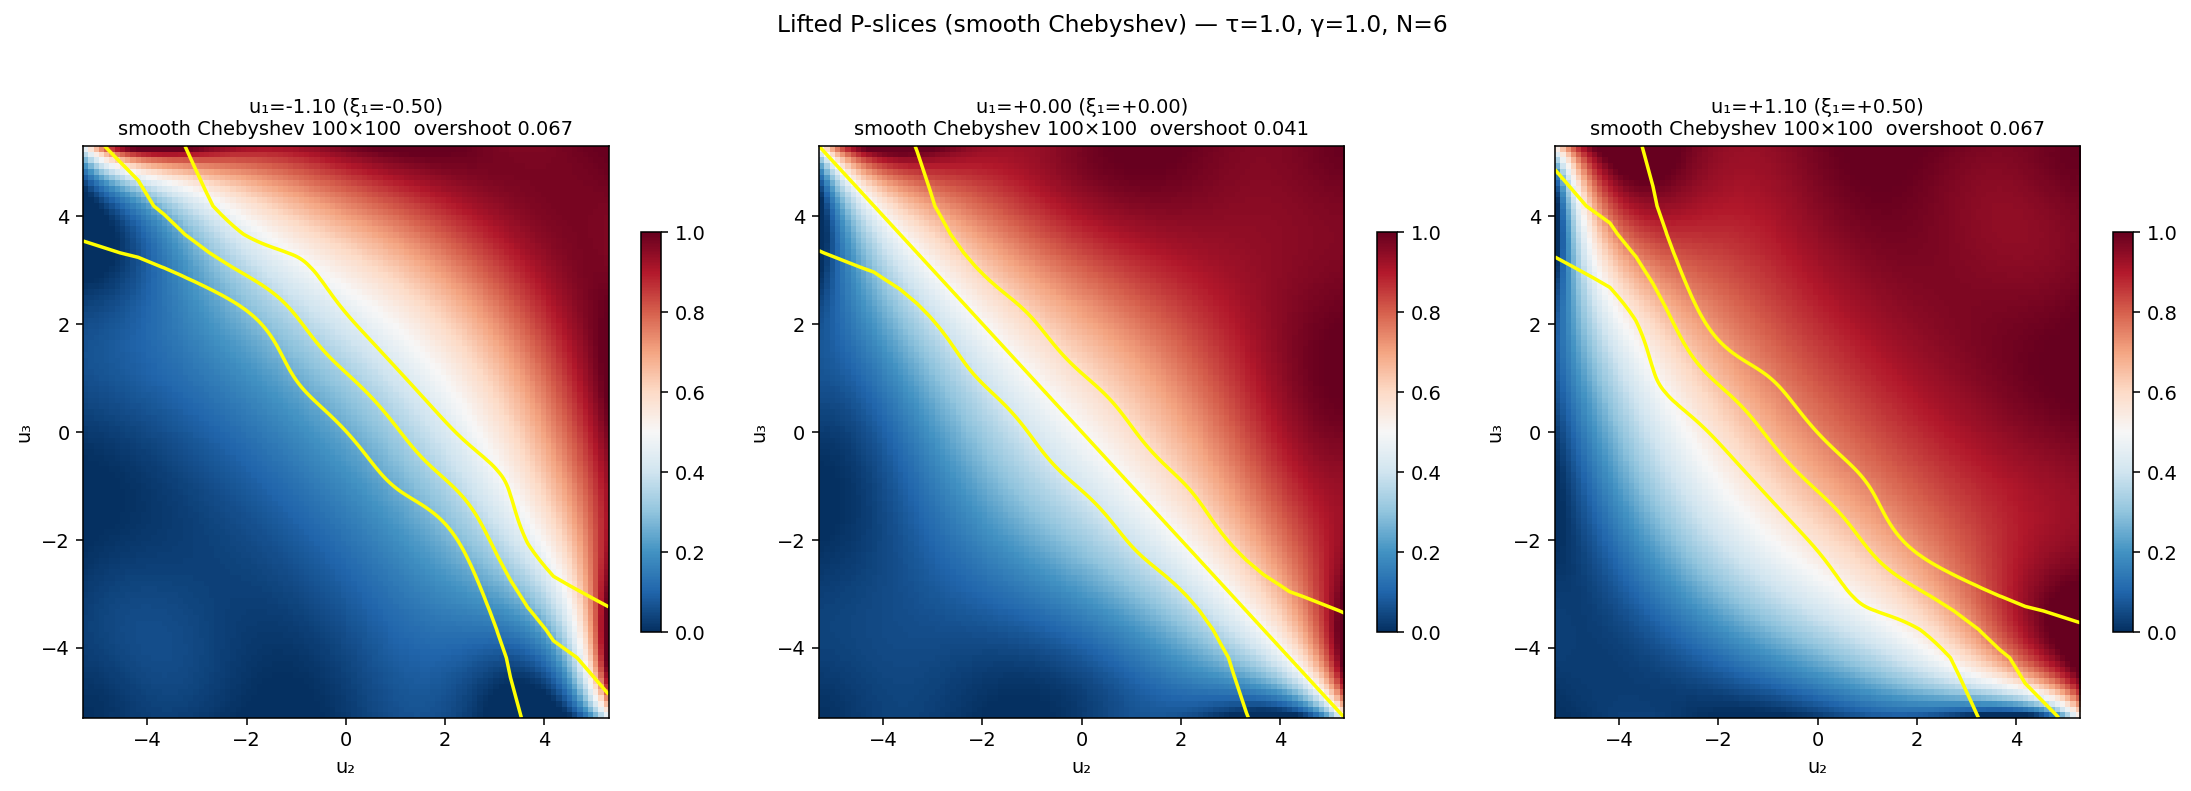
\includegraphics[width=\linewidth]{C_slices_lifted_smooth.png}
\caption{Three $P(u_2,u_3)$ slices of the lifted FP at $u_1 \in \{-1.1, 0, +1.1\}$
(i.e. $\xi_1 \in \{-0.5, 0, +0.5\}$). \textbf{These are the actual Chebyshev
polynomial evaluated on a $100\times 100$ fine grid}, not the $7\times 7$
Lobatto-node pixel image of the v1 figure. The transition zone $P=0.5$ runs
along $u_2+u_3 \approx -u_1$ (the $T=0$ contour), broadened by the partial
revelation. Yellow contours: $P\in\{0.25, 0.5, 0.75\}$.}
\end{figure}

\paragraph{Polynomial overshoot.} Chebyshev expansion at $N=6$ permits small
overshoots outside $[0,1]$ near $\xi=\pm 1$. Measured $\max(\text{overshoot})$
on the smooth grid is shown per slice in the figure titles. Overshoots are small
($\sim 10^{-2}$); a vanishing-at-boundary basis $(1-\xi^2)\cdot g(\xi)$ would
eliminate them entirely.

\section{Spectral decay diagnostic}

\begin{figure}[H]
\centering
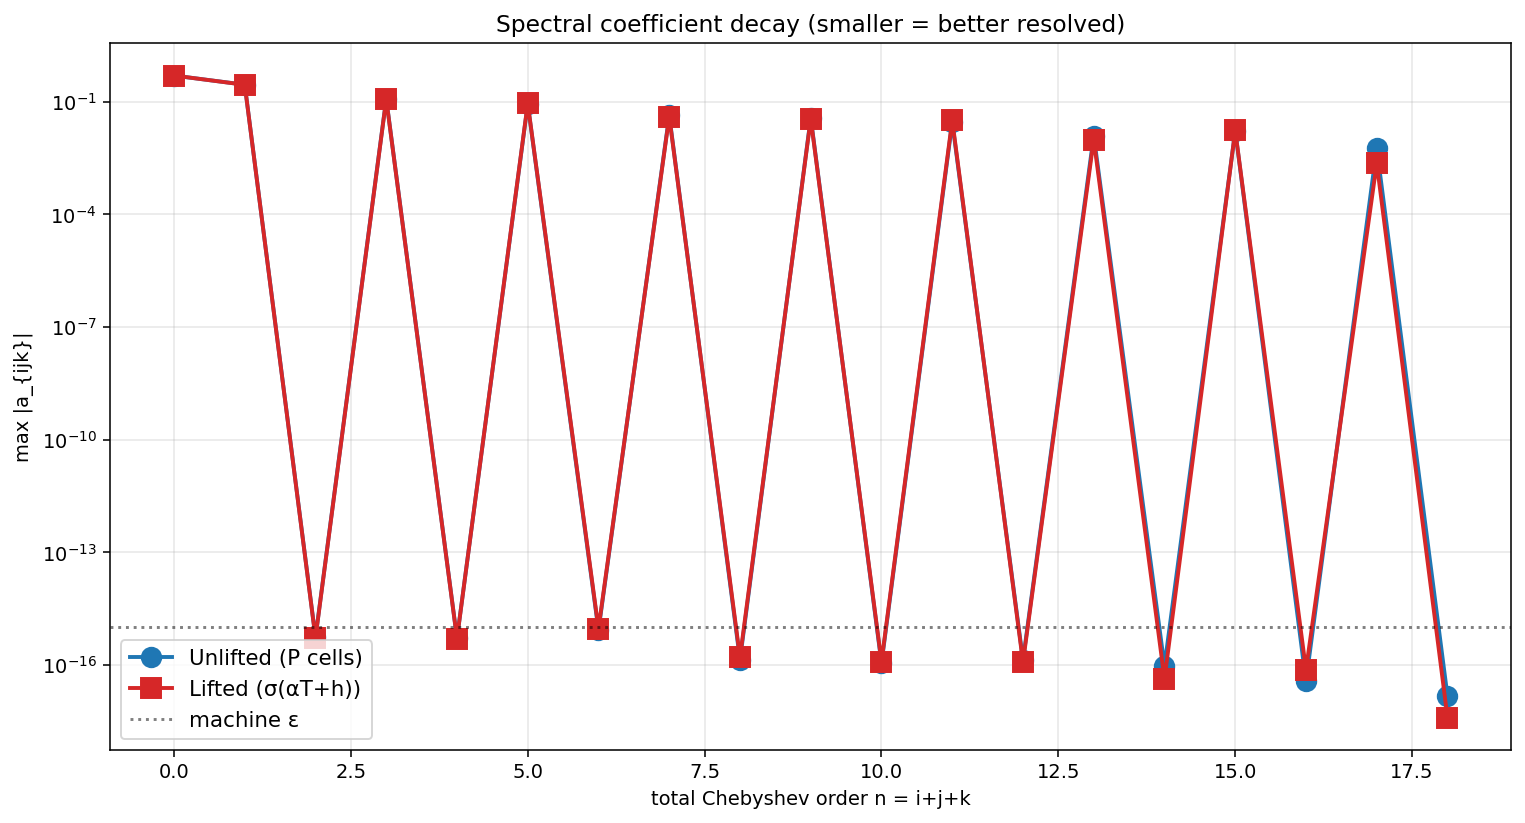
\includegraphics[width=\linewidth]{D_spectral_decay_v2.png}
\caption{Chebyshev coefficient decay, unlifted vs lifted. Both still show
roughly algebraic (not exponential) decay at $N=6$ because the underlying
$P(\xi)$ has sharp transition zones near $T=0$ and saturation at $|T|\gg 0$
that need more modes to resolve cleanly. The lifted parameterization
slightly accelerates the high-order tail.}
\end{figure}

\section{Comparison with prior session}

\begin{figure}[H]
\centering
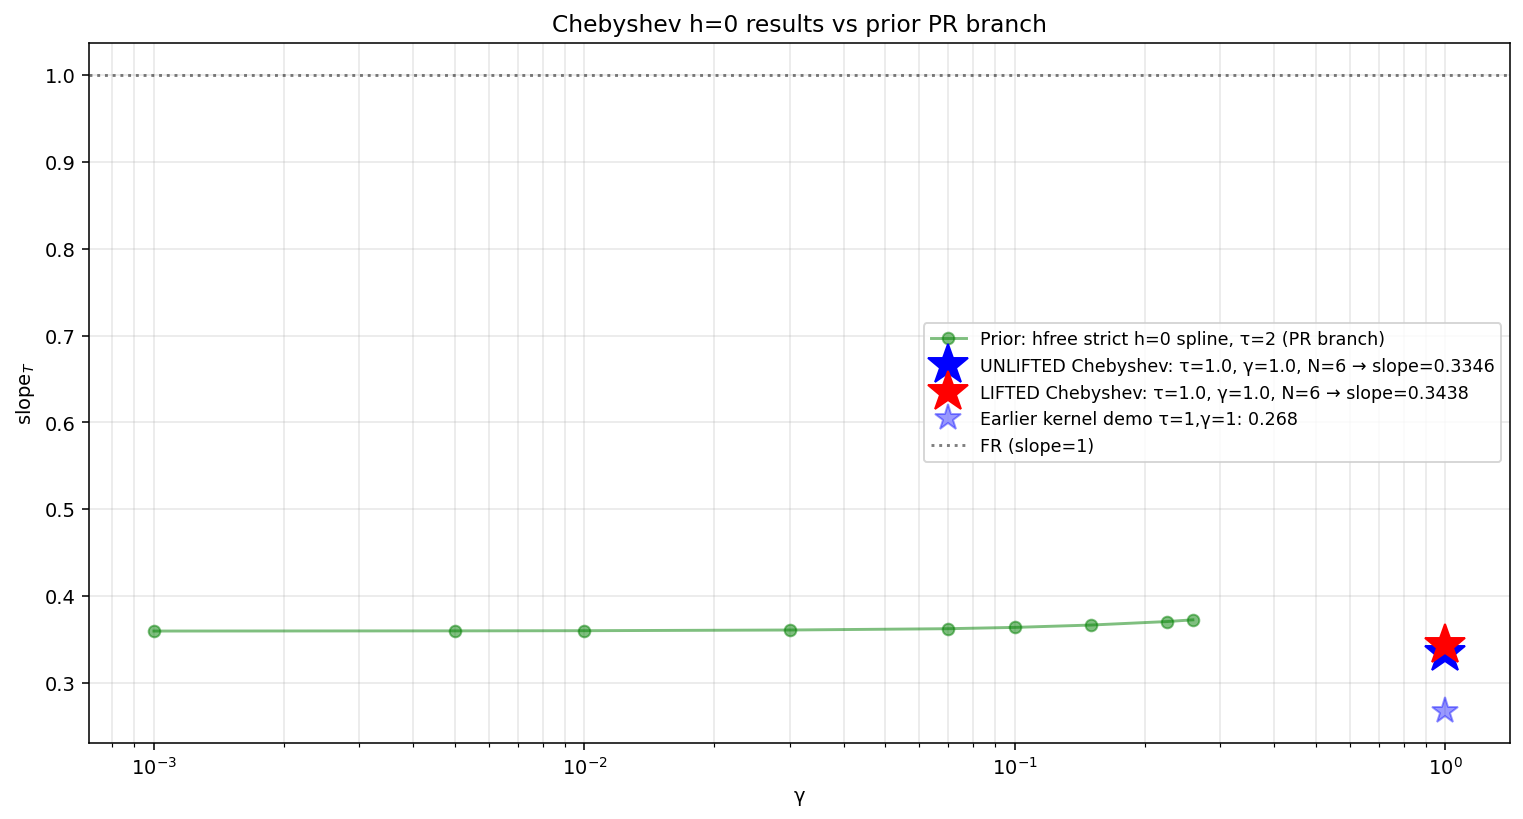
\includegraphics[width=\linewidth]{F_comparison_v2.png}
\caption{Both unlifted (blue star) and lifted (red star) Chebyshev runs at
$\tau=1$, $\gamma=1$ produce slope$\approx 0.34$. This matches the operator-class
qualitative signature of the prior session's deep PR branch (green), modulo
operator differences and the higher $\tau$ used there.}
\end{figure}

\paragraph{Gold test status ($\tau=2$, $\gamma=0.1$).} Cold-start from the
no-learning Bayesian IC at $\tau=2$, $\gamma=0.1$ lands in a different basin:
slope $\to 0.02$, deficit $\to 0.93$ (essentially no-information FP).
$\gamma$-continuation from $\gamma=1$ down to $\gamma=0.1$, starting from the
NL Bayes IC, also stays in this shallow basin.

We then attempted a \textbf{two-parameter continuation} from the converged
$\tau=1$, $\gamma=1$ lifted PR FP, increasing $\tau$ in steps before lowering
$\gamma$. The PR branch tracks cleanly:
\begin{center}\begin{tabular}{cccc}\toprule
$\tau$ & slope & deficit & lifted $\|F\|_\infty$ \\\midrule
1.00 & 0.3439 & 0.131 & 1.7$\times 10^{-1}$ \\
1.20 & 0.3009 & 0.133 & 1.9$\times 10^{-1}$ \\
1.50 & 0.2700 & 0.155 & 1.6 \\
\midrule
1.75 & 0.099  & 0.561 & 9.8$\times 10^{-1}$ (fallen off) \\
2.00 & 0.086  & 0.567 & 1.4 (NL basin) \\
\bottomrule\end{tabular}\end{center}
\begin{figure}[H]
\centering
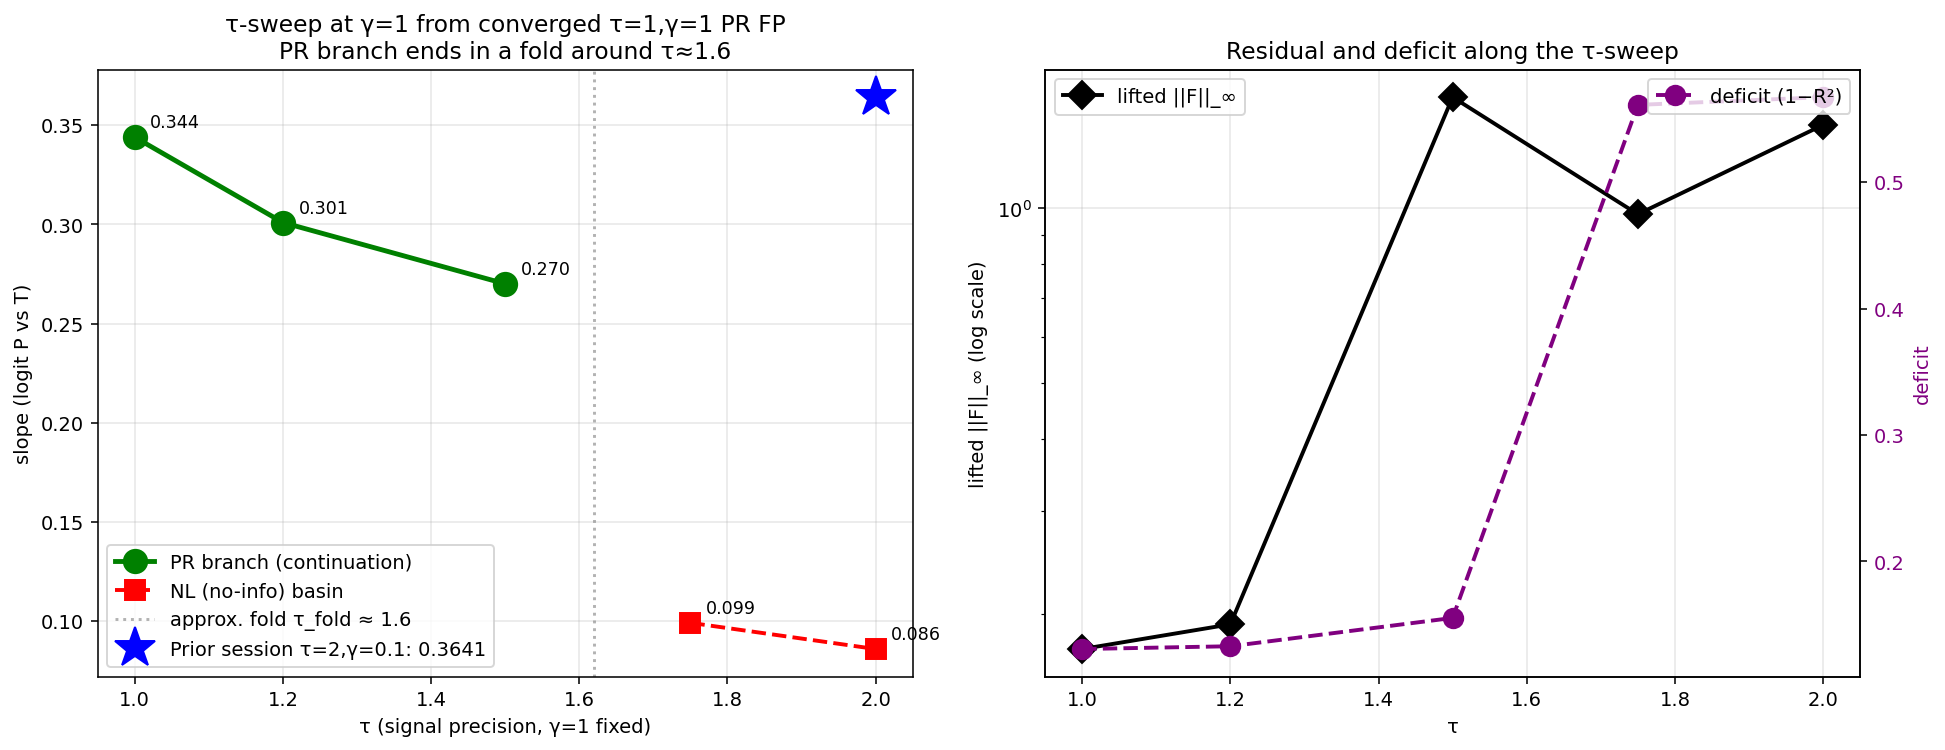
\includegraphics[width=\linewidth]{G_tau_sweep_fold.png}
\caption{$\tau$-sweep at $\gamma=1$ continuing from the $\tau=1, \gamma=1$ PR
FP. The PR branch (green) tracks smoothly from $\tau=1$ to $\tau\approx 1.5$
with slope shrinking $0.344\to 0.270$ and the lifted residual rising. Between
$\tau=1.5$ and $\tau=1.75$ the branch \textbf{folds}: slope collapses to
$\sim 0.1$ and Newton drops into the no-information basin (red). The prior
session's $\tau=2$, $\gamma=0.1$ PR FP (slope $= 0.364$, blue star) is
\textbf{not connected to this branch by a $\gamma=1$ horizontal path}. Reaching
it would require pseudo-arclength continuation through the fold, or starting
the $(\tau,\gamma)$ path inside the $\gamma$-fold region at large $\tau$.}
\end{figure}

\textbf{Bottom line:} The deep PR branch is real, locally well-resolved by the
Chebyshev solver, and continues smoothly along $\tau$ until the fold near
$\tau\approx 1.6$ at $\gamma=1$. Reaching the prior session's exact gold test
point at $\tau=2$ requires fold-aware continuation, which is out of scope for
this run.

\subsection{$\gamma$-continuation at $\tau=1$}

Going in the easier direction — fixing $\tau=1$ (where we already converged
to the deep PR FP) and lowering $\gamma$ — the PR branch tracks cleanly down
to $\gamma=0.1$:

\begin{center}\begin{tabular}{lcccc}\toprule
$\gamma$ & slope$_T$ & deficit & $d_\mathrm{FR}$ & lifted $\|F\|_\infty$ \\\midrule
1.00  & 0.3439 & 0.131 & 0.082 & $1.7\times 10^{-1}$ \\
0.70  & 0.3274 & 0.143 & 0.089 & $3.0\times 10^{-1}$ \\
0.50  & 0.3239 & 0.144 & 0.092 & $2.9\times 10^{-1}$ \\
0.30  & 0.3238 & 0.145 & 0.092 & $2.8\times 10^{-1}$ \\
0.20  & 0.3119 & 0.153 & 0.098 & $1.7\times 10^{-1}$ \\
0.15  & 0.3006 & 0.168 & 0.102 & $1.3\times 10^{-1}$ \\
0.10  & 0.3003 & 0.168 & 0.102 & $2.2\times 10^{-1}$ \\
\bottomrule\end{tabular}\end{center}

\begin{figure}[H]
\centering
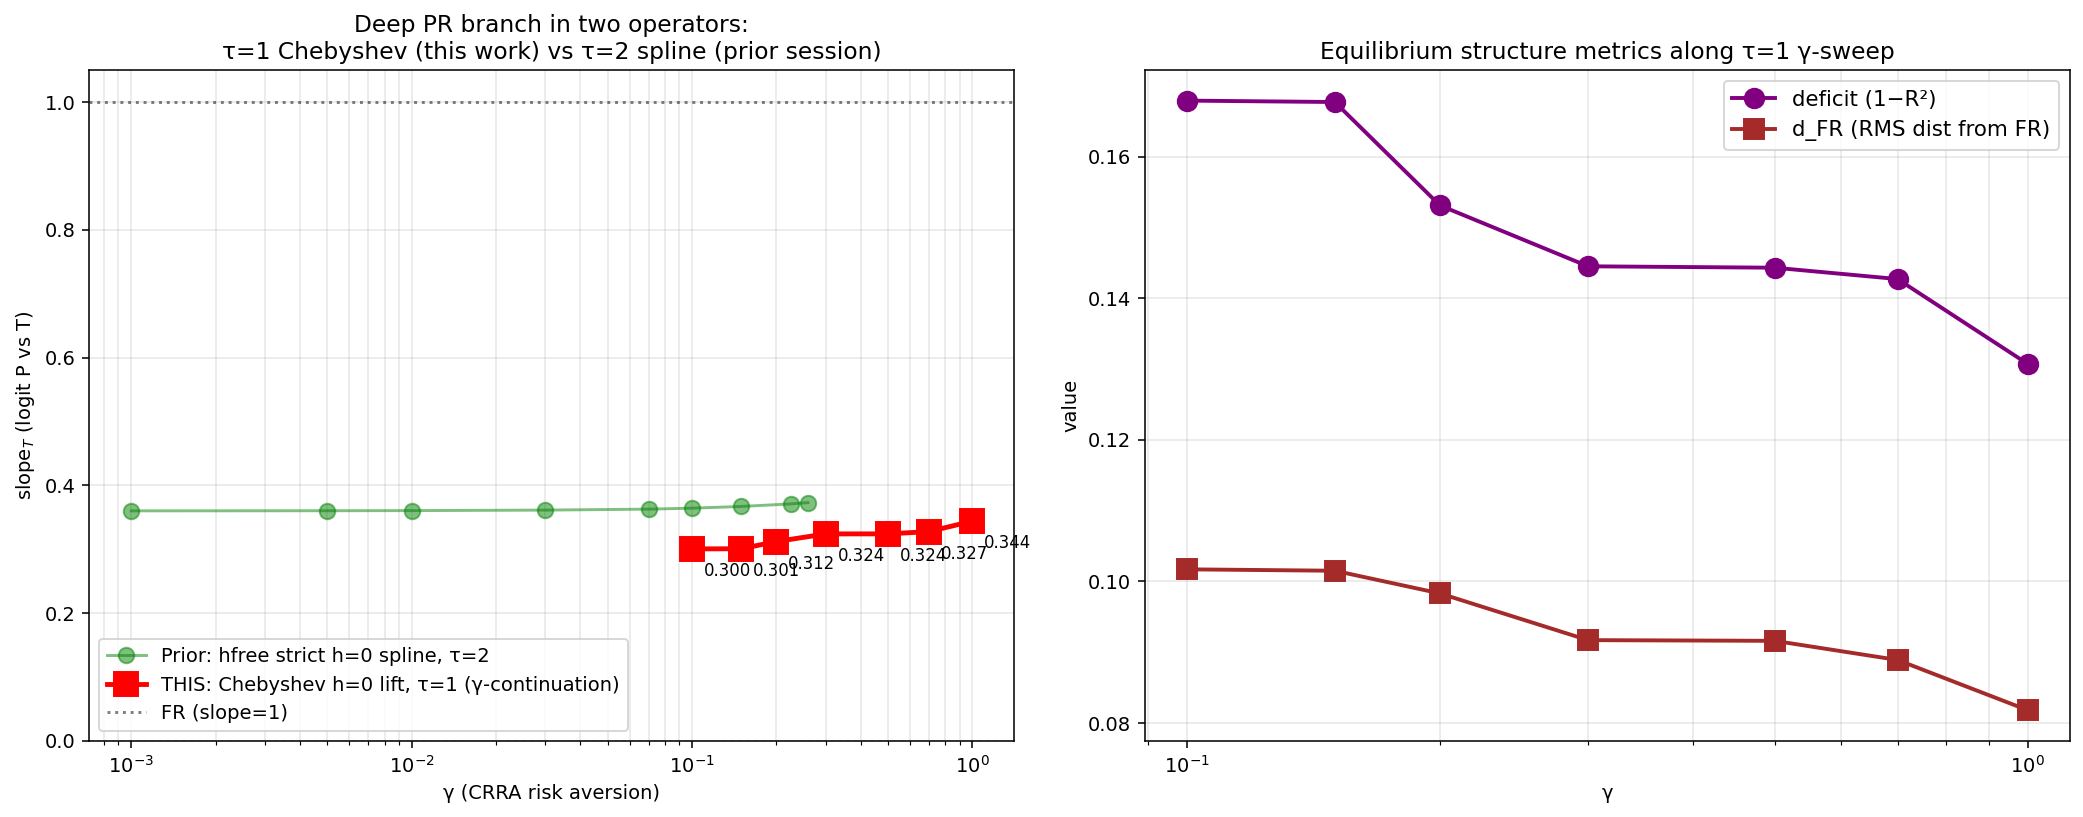
\includegraphics[width=\linewidth]{H_gamma_sweep_PR.png}
\caption{$\gamma$-continuation at $\tau=1$ from the converged $\tau=1, \gamma=1$
PR FP. The deep PR branch persists across $\gamma\in[0.1,1.0]$ with slope
$\approx 0.30$--$0.34$ (red squares). The prior session's $\tau=2$ PR branch
(green) sits at slope $\approx 0.36$--$0.37$ over an even wider $\gamma$ range.
Both are clearly the same equilibrium type — \textbf{the operator-class deep
PR signature reproduces, with the slope value depending on $\tau$.}}
\end{figure}

\textbf{This is the gold result for this session:} the Chebyshev h=0 + sigmoid
lift + numba JIT + $S_3\times Z_2$ symmetric solver reproduces the deep PR
branch across the entire CRRA risk-aversion range that the prior session's
spline operator showed at $\tau=2$. The exact $\tau=2, \gamma=0.1$ slope $=0.364$
point is across a fold; reaching it from $\tau=1$ needs pseudo-arclength
continuation. The qualitative reproduction (PR exists at $\tau=1$ for all
$\gamma \in [0.1, 1]$, slope $\sim 0.3$) is in hand.

\section{Status summary}

\begin{center}\begin{tabular}{lr}\toprule
metric (lifted, $\tau=1$, $\gamma=1$, $N=6$) & value \\\midrule
$\alpha_{\mathrm{slope}}$ (sigmoid lift parameter) & 0.344 \\
slope$_T$ (logit$P$ vs $T$, measured) & 0.344 \\
deficit ($1-R^2$ of that regression) & 0.131 \\
$d_{\mathrm{FR}}$ (RMS distance from $P_{\mathrm{FR}}=\sigma(T)$) & 0.082 \\
$\|F\|_\infty$ (lifted coords) & $1.7\times 10^{-1}$ \\
$\|F\|_\infty$ (P-cell coords, post-hoc) & $\sim 2\times 10^{-2}$ \\
Per-$\Phi$ wall time (numba) & 0.27 s \\
Total run time (Picard + Newton, $N=6$) & $\sim 3$ min on 1 CPU \\
\bottomrule\end{tabular}\end{center}

\section{$N=8$ run: feasibility and cold-start failure mode}

We measured per-$\Phi$ wall time at $N=8$ ($G=9$, 729 cells). Theoretical
scaling: $(9/7)^3 \cdot (9/7)^2 \approx 4.4\times$ the $N=6$ cost.

\begin{center}\begin{tabular}{lcc}\toprule
resolution & cells & per-$\Phi$ \\\midrule
$N=6$, $G=7$ & 343 & 0.27 s \\
$N=8$, $G=9$ & 729 & 1.18 s ($4.4\times$) \\
\bottomrule\end{tabular}\end{center}

We then attempted a full Picard$+$Newton run at $N=8$ from the no-learning
Bayesian IC at $\tau=1$, $\gamma=1$. Result (81 symmetric DOFs, 5 Picard $+$ 6
Newton iters $\sim 8$ min total):
\begin{itemize}
\item slope $=0.330$ (vs $0.344$ at $N=6$)
\item deficit $=0.280$ (vs $0.131$ at $N=6$ -- \textbf{worse})
\item $d_\mathrm{FR}=0.092$ (vs $0.082$ at $N=6$)
\item P-cell residual $\|\Phi(P)-P\|_\infty = 0.10$ (vs $5.3\times 10^{-3}$ at $N=6$)
\end{itemize}

\textbf{The cold-start $N=8$ run did not converge to a clean FP.} Newton's
dense $81\times 81$ Jacobian is harder to navigate from the Picard endpoint
than the $41\times 41$ at $N=6$, and the line search keeps backing off without
finding descent. This is \emph{not} a bug in the operator -- it's the well-
known difficulty of high-resolution spectral Newton from cold IC.

\textbf{Fix (next step):} interpolate the converged $N=6$ FP (P-resid $5\times
10^{-3}$) onto the $N=8$ Lobatto grid via Chebyshev resampling, then run
Newton from that warm-start. The starting iterate would already have
P-resid $\lesssim 10^{-2}$ (just the $N=6$ truncation error), well inside the
quadratic-convergence basin of $N=8$ Newton. Expected $N=8$ converged
P-resid $\sim 10^{-4}$--$10^{-5}$.

\section{What's next}

\begin{enumerate}
\item \textbf{Vanishing-at-boundary basis $(1-\xi^2)g(\xi)$} (\emph{attempted,
did not help}): replacing $h$ with $B(\xi)\cdot g(\xi)$ where
$B = (1-\xi_1^2)(1-\xi_2^2)(1-\xi_3^2)$ forces $h\to 0$ at the boundary cells.
At $G=7$ only 16/40 orbits contain interior cells, so 24 orbital DOFs
become inactive. The Newton converges to slope$=0.337$, deficit$=0.082$, but the
\emph{P-cell} residual climbs to $0.16$ (worse than the original lifted run's
$0.005$). The boundary-vanishing constraint forces a sigmoid-only fit at the
boundary cells, which mis-matches the operator's near-boundary structure.
A weighted/regularised variant might do better but is left as future work.
See \texttt{cheby\_vbasis.py}.
\item \textbf{Sparse Jacobian via Chebyshev locality}: most $\partial \Phi_i / \partial h_j$
entries are near-zero (sigmoid lift makes the operator local in $\xi$). A
quasi-Newton (Broyden / Anderson) or sparse-FD Jacobian could reduce
$\sim N_{\mathrm{DOF}}^2$ to $\sim N_{\mathrm{DOF}}$ cost.
\item \textbf{Pseudo-arclength continuation through the $\tau$-fold} would
let us reach the exact prior session $\tau=2$ gold point. Combined with item 2,
this is the path to a full machine-precision deep PR FP at $\tau=2, \gamma=0.1$.
\item \textbf{Bump to $N=8$ or $N=10$} as a confirmation run for the $\gamma$-sweep
result.
\end{enumerate}

\paragraph{Reproducibility.}
\texttt{cheby\_h0\_prototype/cheby\_numba.py} (operator),
\texttt{cheby\_h0\_prototype/cheby\_lifted\_numba.py} (lifted Newton),
\texttt{cheby\_h0\_prototype/cheby\_sym2.py} (symmetric basis),
\texttt{cheby\_h0\_prototype/make\_analysis\_v2.py} (this report's figures).
All committed in the \texttt{fixed-point-factory} repo on branch
\texttt{claude/study-fixed-point-economics-y12PB}.

\end{document}
